O módulo \texttt{tsp/naive.py} reconstrói, como linha de base, os padrões de
código ingênuo que um LLM tipicamente entrega sem revisão. São eles:
\begin{itemize}
  \item best-first que copia o caminho inteiro em cada filho, testa
    pertinência com \texttt{v in path} em lista ($O(n)$) e recalcula o
    limite do zero em Python puro ($O(n^2)$ por nó);
  \item TATT e Christofides sobre o grafo \emph{completo} do NetworkX
    ($n(n-1)/2$ arestas como dicionários);
  \item circuito euleriano via \texttt{MultiGraph}.
\end{itemize}
O script \texttt{audit\_naive.py} mede as duas versões nas mesmas
condições (Tabelas~\ref{tab:auditoria_aprox} e~\ref{tab:auditoria_bnb},
Figura~\ref{fig:auditoria_mst}).

\paragraph{Aproximativos.} No TATT, trocar o grafo do NetworkX pelo Prim
$O(n^2)$ sobre a matriz deu 89$\times$ menos tempo e 714$\times$ menos
memória em $N=500$ (49~MiB contra 0,07~MiB). No Christofides o ganho de
tempo é pequeno (1,1 a 2,1$\times$), e foi o \emph{profiling por
subrotina} que mostrou por quê: o blossom domina as duas versões. Ele
responde por 81\% do tempo já em $N=25$ e por praticamente 100\% em
$N=1000$ (Figura~\ref{fig:tempo}b). A refatoração reduziu a memória em 3,8
a 7,2$\times$, porque o grafo do matching agora tem só os $k$ vértices
ímpares, e não mais os $n$ vértices. Mais tempo nas outras subrotinas não
mudaria o total: o próximo passo seria um matching em C, ou o guloso, que
custa 2$\times$ mais gap (Seção~\ref{sec:sens}).

\begin{figure}[htb]
\centering
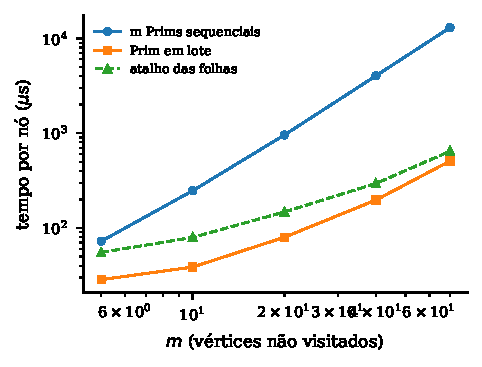
\includegraphics[width=0.5\textwidth]{auditoria_children_mst}
\caption{Tempo para calcular $\mathrm{MST}(R\setminus\{c\})$ para todos os
$m$ filhos de um nó: $m$ execuções sequenciais do Prim, Prim em lote e atalho
das folhas.}\label{fig:auditoria_mst}
\end{figure}

\paragraph{Limites dos filhos no B\&B.} O profiling do B\&B
(Tabela~\ref{tab:perfil}) mostrou que, nas configurações em que a árvore é
grande, 83 a 94\% do tempo vai para o cálculo dos limites dos filhos. Com
Held-Karp e filhos por LB, as árvores são tão pequenas que metade do tempo
vai para o subgradiente na raiz. O Prim em lote foi
25$\times$ mais rápido que $m$ execuções sequenciais em $m=70$ (0,51~ms
contra 12,96~ms). A revisão cruzada sugeriu ainda o \emph{atalho das
folhas}: se $c$ é folha da MST $T$ de $R$, então $T-c$ é MST de $R-c$, e
o limite sai em $O(1)$. A propriedade é verdadeira, e a implementação bate
com o Prim sequencial nos testes. Mesmo assim, ela foi 1,3 a 2,1$\times$
\emph{mais lenta} que o lote para $m\le70$. O atalho exige um Prim extra
com $m$ iterações do interpretador, e nesse tamanho o custo é dominado pelo
número de iterações Python, não pela aritmética, que o NumPy faz em
microssegundos. É um exemplo direto de gargalo teórico que não é o gargalo
prático, por isso a versão em lote continuou como padrão.

\begin{table}[htb]
\centering
\caption{Auditoria dos aproximativos: versão bruta (grafo completo no NetworkX) x refatorada (Prim $O(n^2)$ na matriz, matching só nos vértices ímpares). Tempo: mediana de 3 execuções; memória: pico do tracemalloc.}
\label{tab:auditoria_aprox}
\small
\begin{adjustbox}{max width=\linewidth}
\begin{tabular}{lrlrrrrr}
\toprule
Caso & $N$ & Algoritmo & Tempo bruto (ms) & Tempo ref. (ms) & Speedup & Mem. bruto (MiB) & Mem. ref. (MiB) \\
\midrule
gr24 & 24 & TATT & 0{,}39 & 0{,}08 & 5{,}0$\times$ & 0{,}13 & 0{,}01 \\
gr24 & 24 & Christofides & 1{,}37 & 0{,}66 & 2{,}1$\times$ & 0{,}21 & 0{,}05 \\
att48 & 48 & TATT & 1{,}30 & 0{,}14 & 9{,}0$\times$ & 0{,}46 & 0{,}01 \\
att48 & 48 & Christofides & 9{,}91 & 7{,}02 & 1{,}4$\times$ & 0{,}68 & 0{,}18 \\
st70 & 70 & TATT & 2{,}67 & 0{,}21 & 12{,}7$\times$ & 0{,}90 & 0{,}02 \\
st70 & 70 & Christofides & 11{,}39 & 8{,}08 & 1{,}4$\times$ & 1{,}11 & 0{,}23 \\
random200 & 200 & TATT & 22{,}74 & 0{,}64 & 35{,}5$\times$ & 7{,}78 & 0{,}03 \\
random200 & 200 & Christofides & 155{,}71 & 117{,}47 & 1{,}3$\times$ & 7{,}78 & 1{,}09 \\
random500 & 500 & TATT & 170{,}03 & 1{,}90 & 89{,}4$\times$ & 48{,}94 & 0{,}07 \\
random500 & 500 & Christofides & 2.551{,}72 & 2.221{,}46 & 1{,}1$\times$ & 48{,}94 & 8{,}86 \\
\bottomrule
\end{tabular}
\end{adjustbox}
\end{table}

\begin{table}[htb]
\centering
\caption{Auditoria do B\&B (limite de 30 s por execução; todas as variantes com o mesmo warm-start, vizinho mais próximo, e o mesmo teto de 2 milhões de nós abertos). B/nó aberto: pico de memória dividido pelo máximo de nós abertos, ambos da mesma execução com tracemalloc.}
\label{tab:auditoria_bnb}
\small
\begin{adjustbox}{max width=\linewidth}
\begin{tabular}{llcrrrr}
\toprule
Instância & Variante & Status & Nós exp. & Tempo (s) & Pico (MiB) & B/nó aberto \\
\midrule
burma14 & bruto: best-first, cópias, LB em Python & ótimo & 483.341 & 18{,}13 & 101{,}2 & 259 \\
burma14 & bruto, GC desligado & ótimo & 483.341 & 17{,}78 & 101{,}3 & 260 \\
burma14 & best-first refatorado & ótimo & 237.333 & 3{,}66 & 98{,}1 & 273 \\
burma14 & best-first refatorado, GC desligado & ótimo & 237.333 & 3{,}46 & 98{,}1 & 273 \\
burma14 & DFS, 2 menores arestas & ótimo & 278.533 & 3{,}35 & 0{,}0 & -- \\
burma14 & DFS, 1-árvore & ótimo & 7.772 & 0{,}24 & 0{,}0 & -- \\
burma14 & DFS, Held-Karp & ótimo & 12 & 0{,}00 & 0{,}0 & -- \\
ulysses16 & bruto: best-first, cópias, LB em Python & memória & 337.320 & 27{,}26 & 104{,}0 & 257 \\
ulysses16 & bruto, GC desligado & memória & 337.320 & 25{,}18 & 103{,}9 & 257 \\
ulysses16 & best-first refatorado & memória & 311.106 & 6{,}84 & 365{,}7 & 268 \\
ulysses16 & best-first refatorado, GC desligado & memória & 311.106 & 5{,}75 & 368{,}4 & 268 \\
ulysses16 & DFS, 2 menores arestas & timeout & 2.497.158 & 30{,}00 & 0{,}0 & -- \\
ulysses16 & DFS, 1-árvore & timeout & 1.092.828 & 30{,}00 & 0{,}0 & -- \\
ulysses16 & DFS, Held-Karp & ótimo & 14 & 0{,}01 & 0{,}0 & -- \\
gr17 & bruto: best-first, cópias, LB em Python & timeout & 327.115 & 30{,}42 & 94{,}9 & 260 \\
gr17 & bruto, GC desligado & timeout & 347.969 & 30{,}45 & 95{,}2 & 260 \\
gr17 & best-first refatorado & memória & 419.819 & 8{,}89 & 323{,}4 & 270 \\
gr17 & best-first refatorado, GC desligado & memória & 419.819 & 7{,}72 & 322{,}0 & 270 \\
gr17 & DFS, 2 menores arestas & timeout & 2.426.378 & 30{,}00 & 0{,}0 & -- \\
gr17 & DFS, 1-árvore & ótimo & 293.064 & 10{,}62 & 0{,}0 & -- \\
gr17 & DFS, Held-Karp & ótimo & 15 & 0{,}00 & 0{,}0 & -- \\
\bottomrule
\end{tabular}
\end{adjustbox}
\end{table}


\paragraph{Estratégia da árvore: best-first $\times$ DFS.} Com o mesmo
limite fraco (duas menores arestas), o mesmo warm-start e o mesmo teto de
nós abertos, o best-first refatorado resolveu o burma14 em 3,7~s, contra
18,1~s da versão bruta. Ele expandiu metade dos nós (237 mil contra 483
mil), porque o limite refatorado restringe as arestas livres das pontas do
caminho aos vértices não visitados. Nas duas versões, porém, cada nó aberto
custa cerca de 260 a 270~bytes, e a fila chega a centenas de MiB. No
ulysses16 e no gr17, o best-first estourou o teto de 2 milhões de nós
abertos (320 a 370~MiB) em menos de 10~s. A DFS com o mesmo limite usou
0,03~MiB nas três instâncias. Por isso a DFS é a estratégia padrão: a
memória cai de exponencial para $O(n^2)$, e a perda (expandir nós que o
best-first não expandiria) é compensada por um bom limite. Com Held-Karp, a
DFS resolveu as três instâncias expandindo 12 a 15 nós em menos de 10~ms.
Para o best-first, guardar o caminho como lista encadeada (filho em $O(1)$)
reduziu o custo por nó de $\approx$340 para $\approx$270~bytes. O restante
é o custo fixo de uma tupla Python com 6 campos.
